%\documentclass[10pt,handout]{beamer}
\documentclass[10pt]{beamer}
\usepackage[english]{babel} % Anpassa efter svenska. Ger svensk logga.
\usepackage[utf8]{inputenc} % Anpassa efter linux
\usepackage{graphicx}
\usepackage{../common/beamerthemeUppsala}
%\usecolortheme{UU} % Anpassa efter UU:s frger och logga
%\hypersetup{pdfpagemode=FullScreen} % Adobe Reader ska ppna fullskrm
\setbeamertemplate{itemize items}[circle]

% \usepackage{beamerthemesplit}
\usepackage{amsmath}
\usepackage{amssymb}
% \usepackage{graphics}
% \usepackage{graphicx}
% \usepackage{epsfig}
% \usepackage[latin1]{inputenc}
 \usepackage{color}
% \usepackage{fancybox}
% \usepackage{psfrag}
% \usepackage[english]{babel}
 \setbeamertemplate{footline}{\hfill\insertframenumber/\inserttotalframenumber}


%library(tinytex)
%tlmgr_install('csquotes')
%\usepackage{csquotes}

% Read in commands
% Course settings
\newcommand{\currentsemester}{Autumn 2024}

% New commands
\newcommand{\bfm}[1]   {\mbox{\boldmath{${#1}$}}}
\newcommand{\Prob}   {\mbox{\textnormal{P}}}
\newcommand{\uured}[1]{\textcolor{uured}{#1}}

% Eqds
\def\eqd{\,{\buildrel d \over =}\,}

% Math operators
\DeclareMathOperator{\E}{\mathbb{E}}
\DeclareMathOperator{\V}{\mathbb{V}}


%%%%%%%%%%%%%%%%%%%%%%%%%%%%%%%%%%%%%%%%%%%%%%%%%%%%%%%%%%%%%%%%%%

\setlength{\parskip}{3mm}
\title[]{{\color{black}Machine learning -- Block 4}}
\author[]{M{\aa}ns Magnusson\\Department of Statistics, Uppsala University}
\date{\currentsemester}


\begin{document}

\frame{\titlepage
% \thispagestyle{empty}
}

%%%%%%%%%%%%%%%%%%%%%%%%%%%%%%%%%%%%%%%%%%%%%%%%%%%%%%%%%%%%%%%%%%


\begin{frame}{This week's lecture}
\begin{itemize}
\item Previous assignments
\item The Mini-Project and Master Thesis Projects
\item Convolutional Neural Networks
\item Transfer Learning
\end{itemize}
\end{frame}



%%%%%%%%%%%%%%%%%%%%%%%%%%%%%%%%%%%%%%%%%%%%%%%%%%%%%%%%%%%%%%%%%%

\section{Previous assignments}

\begin{frame}{Assignment 3: Evaluation}

\begin{itemize}
\item ?
\end{itemize}

\end{frame}


\section{The Mini-Project}


\begin{frame}{Mini-project}

\begin{itemize}
\item Time to start think about the project.\pause
\item {\color{uured} Supervised} problem of choice on {\color{uured} real data}.\pause
\item 2-3 students.\pause
\item Supply a {\color{uured} project proposal} of data and problem at the end of \emph{15th of December 23.59}.
\item \emph{Hint!} Submit page 1-1.5 of the project as project proposal.
\item Deadline is after all lectures on supervised learning\pause
\item Feel free to combine it with your master thesis project!\pause
\item Check with me if you have questions.
\item The project should result in a 4 page report (PDF) using the {\color{uured} ICML LaTeX template}.
\end{itemize}
\end{frame}


\section{Introduction}
\frame{\sectionpage}

\frame{\frametitle{Convolutional Neural Networks}

\begin{itemize}
\item \uured{Acknowledgements}: Anders Eklund, Link\"{o}ping University.\pause
\item \uured{Convolutional} Neural Networks are behind great progress in the 2010s.
\item It has revolutionized \uured{Computer Vision}.
\item Also called: ConvNets, Convolutional nets, Convolutional networks
\end{itemize}

\begin{figure}[h]
\caption{ImageNet performance (Roessler, 2019)}
\centering
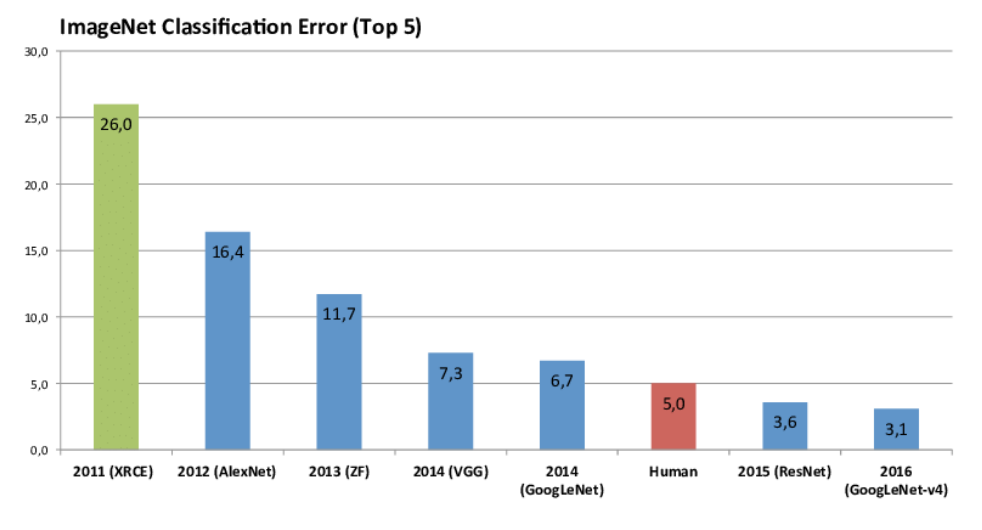
\includegraphics[width=0.8\textwidth]{fig/imageNet.png}
\end{figure}
\pause

}


\frame{\frametitle{Convolutional Neural Networks}

\begin{itemize}
\item Special architecture that works well for data with a \uured{grid structure}
\begin{enumerate}
\item 1D-grids: Time series\pause
\item 2D-grids: Gray-scale Images (pixels)\pause
\item 3D-grids: Color Images (pixels and chanels)\pause
\item 4D-grids: Color Video (pixels, chanels, frames)
\end{enumerate}
\end{itemize}

}

\frame{\frametitle{Computer Vision}

\begin{itemize}
\item Problems
\begin{itemize}
\item Image Classification\pause
\item Image Segmentation\pause
\item Object Detection\pause
\item Object Localization\pause
\end{itemize}
\item {\color{uured} Focus}: 2D and 3D data\pause
\item Very Large Datasets:
\begin{itemize}
\item ImageNet: 14M Images, 20k classes, 1M bounding boxes
\end{itemize}
\pause
\item Many different pre-trained models (e.g. VGG16)
\end{itemize}
}

\frame{\frametitle{Example: Object Detection}
\begin{figure}[h]
\centering
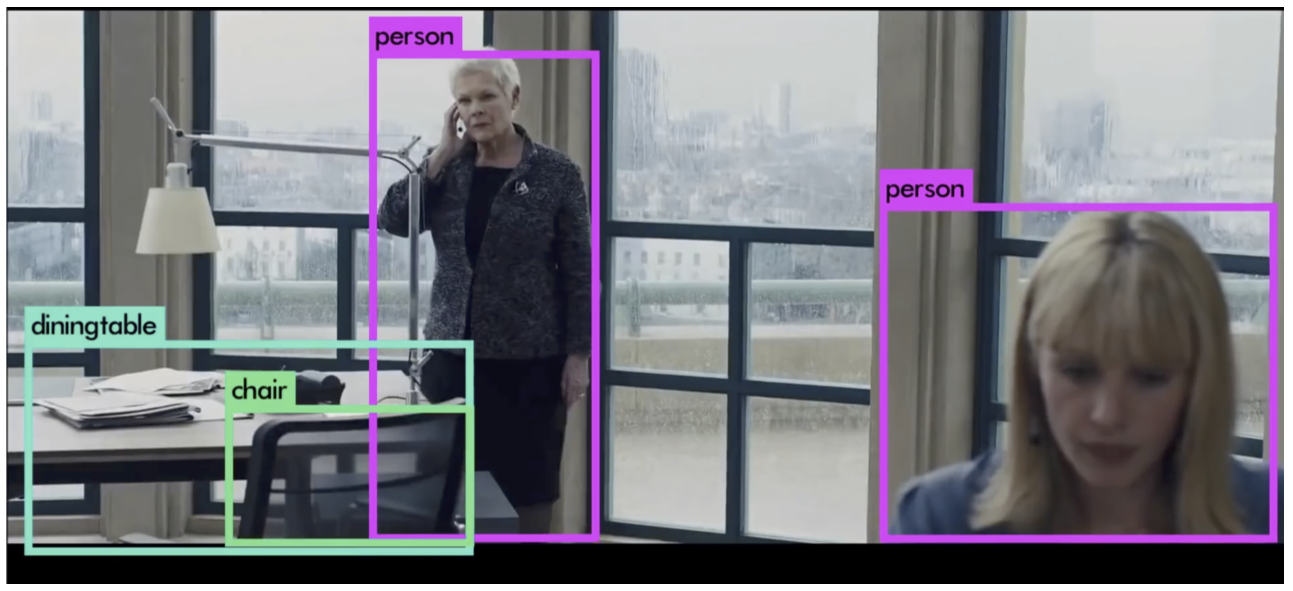
\includegraphics[width=0.8\textwidth]{fig/object_detection.png}
\caption{Object detection (see \href{https://www.youtube.com/watch?v=VOC3huqHrss}{https://www.youtube.com/watch?v=VOC3huqHrss}) }
\end{figure}
}

\frame{\frametitle{Example: Pneumonia detection}
\begin{figure}[h]
\centering
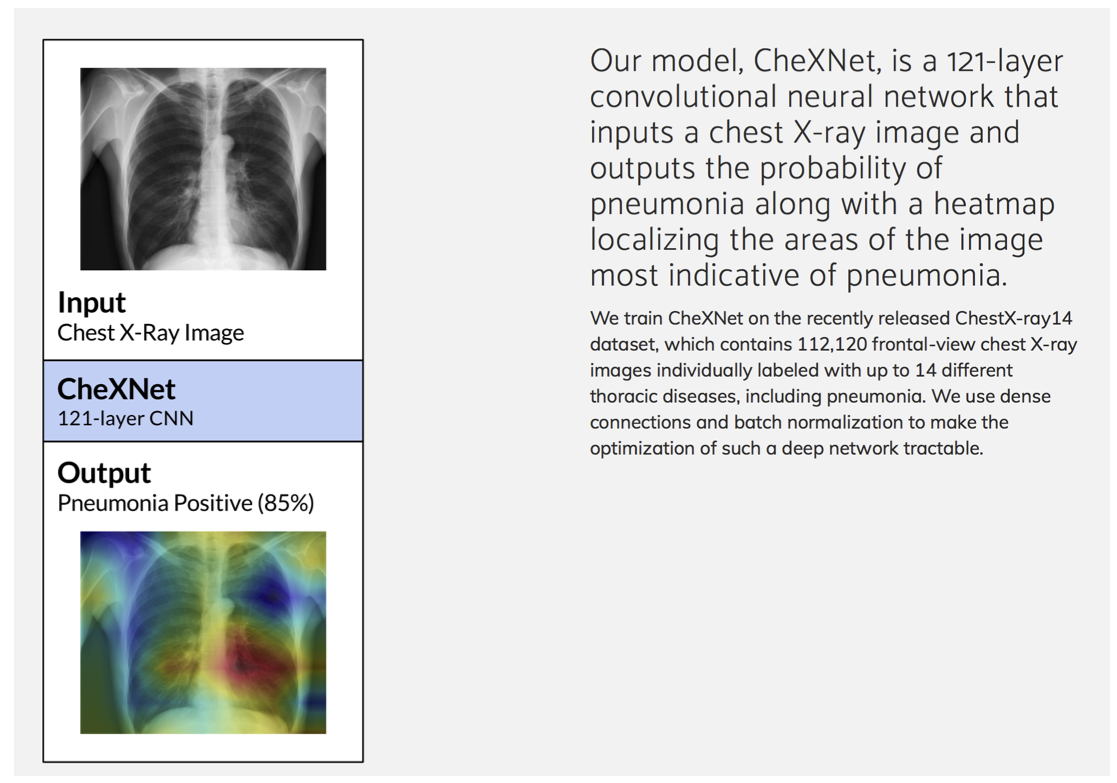
\includegraphics[width=0.8\textwidth]{fig/chexnet.png}
\caption{Rajpurkar et al. (2017). Chexnet: Radiologist-level pneumonia detection on chest x-rays with deep learning. arXiv preprint arXiv:1711.05225.}
\end{figure}
}

\frame{\frametitle{Example: Fracture detection}
\begin{figure}[h]
\centering
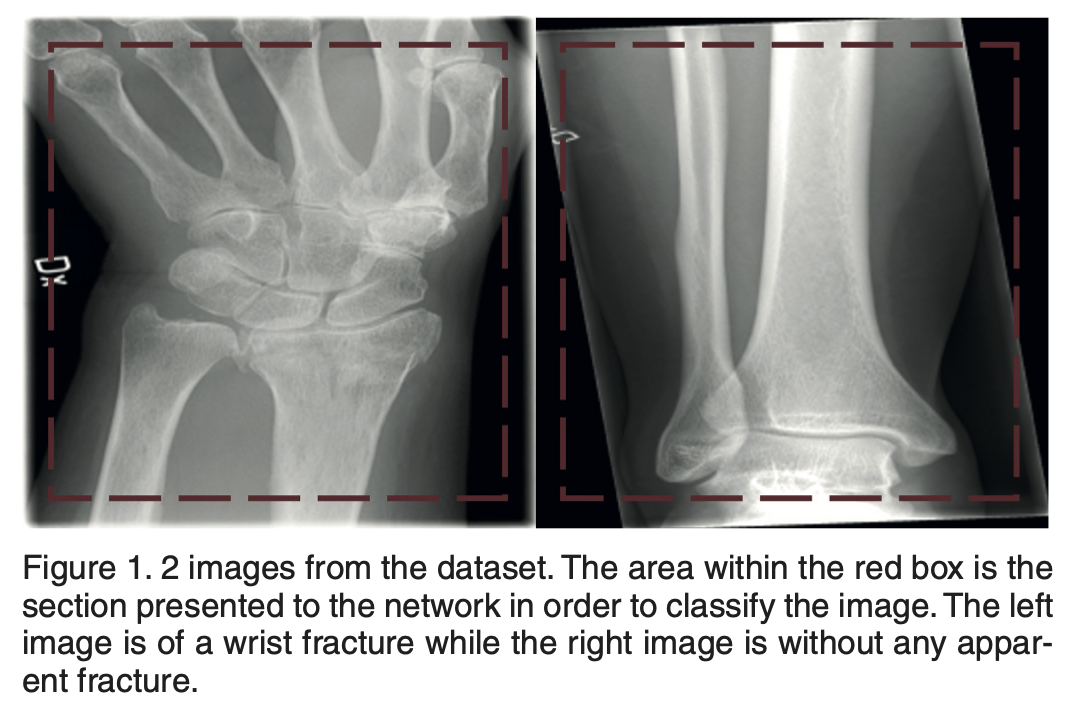
\includegraphics[width=0.8\textwidth]{fig/fractures.png}
\caption{Olczak et al, (2017) Artificial intelligence
for analyzing orthopedic trauma radiographs, Acta Orthopaedica, 88:6, 581-586}
\end{figure}
}


\frame{\frametitle{What is an Image?}

\begin{itemize}
\item 2-dimensional object
\item Each pixel has:
\begin{enumerate}
\item a coordinate
\item a value (light intensity)
\end{enumerate}\pause
\item {\color{uured} Grayscale}: single channel
\item {\color{uured} Color}: three channel (RGB)\pause
\item Spatial and hiearchical correlation structures
\end{itemize}
}

\frame{\frametitle{MNIST example}

\begin{figure}[h]
\centering

\includegraphics[width=0.7\textwidth]{fig/MNIST_example.png}
\caption{Example from the MNIST dataset (28 by 28 pixels)}
\end{figure}

}

\frame{\frametitle{How to train models for images?}

\begin{itemize}
\item We want to learn {\color{uured} representations} of parts of images
\begin{figure}[h]
\centering
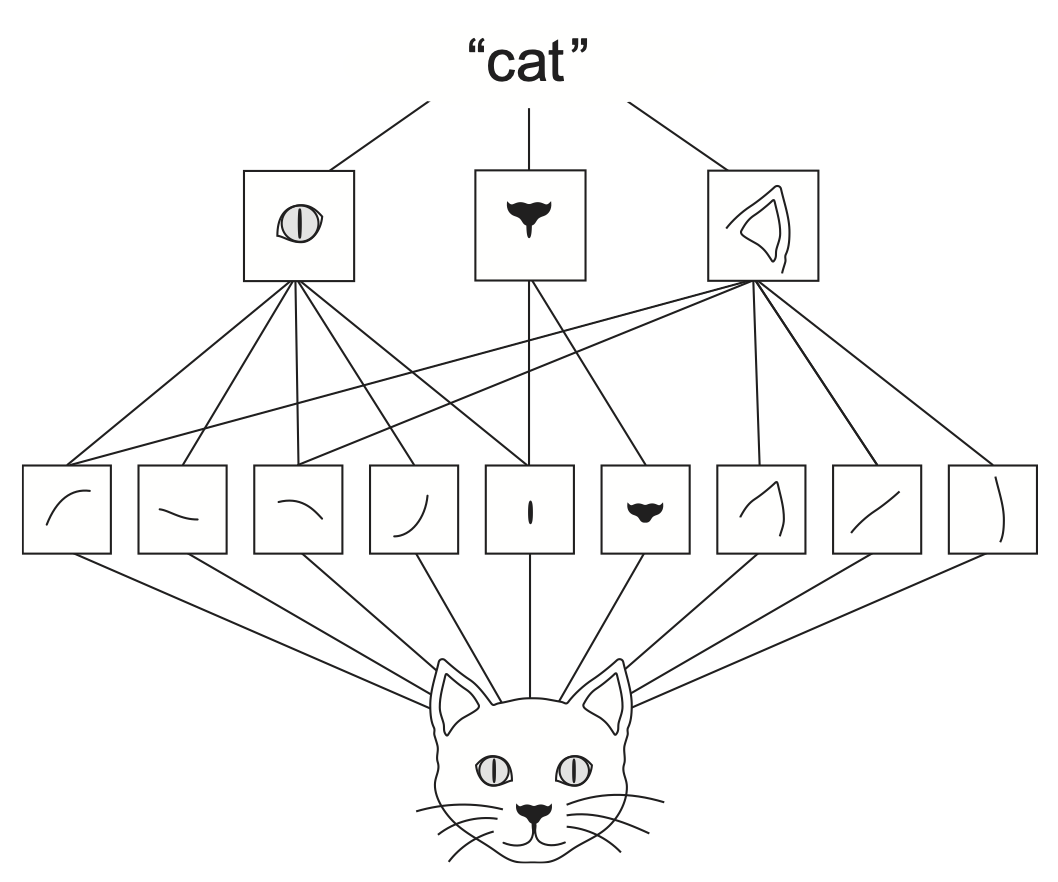
\includegraphics[width=0.7\textwidth]{fig/DLR_Fig_5_2_cat.png}
\caption{The representations of a cat (Chollet and Allair, 2018, Fig 5.2)}
\end{figure}
\pause
\item CNN uses \uured{Convolutional Layers} to learn \uured{parameter efficient} representations
\end{itemize}

}


\frame{\frametitle{Learning Representations for Images (again)}

\begin{figure}[h]
\centering
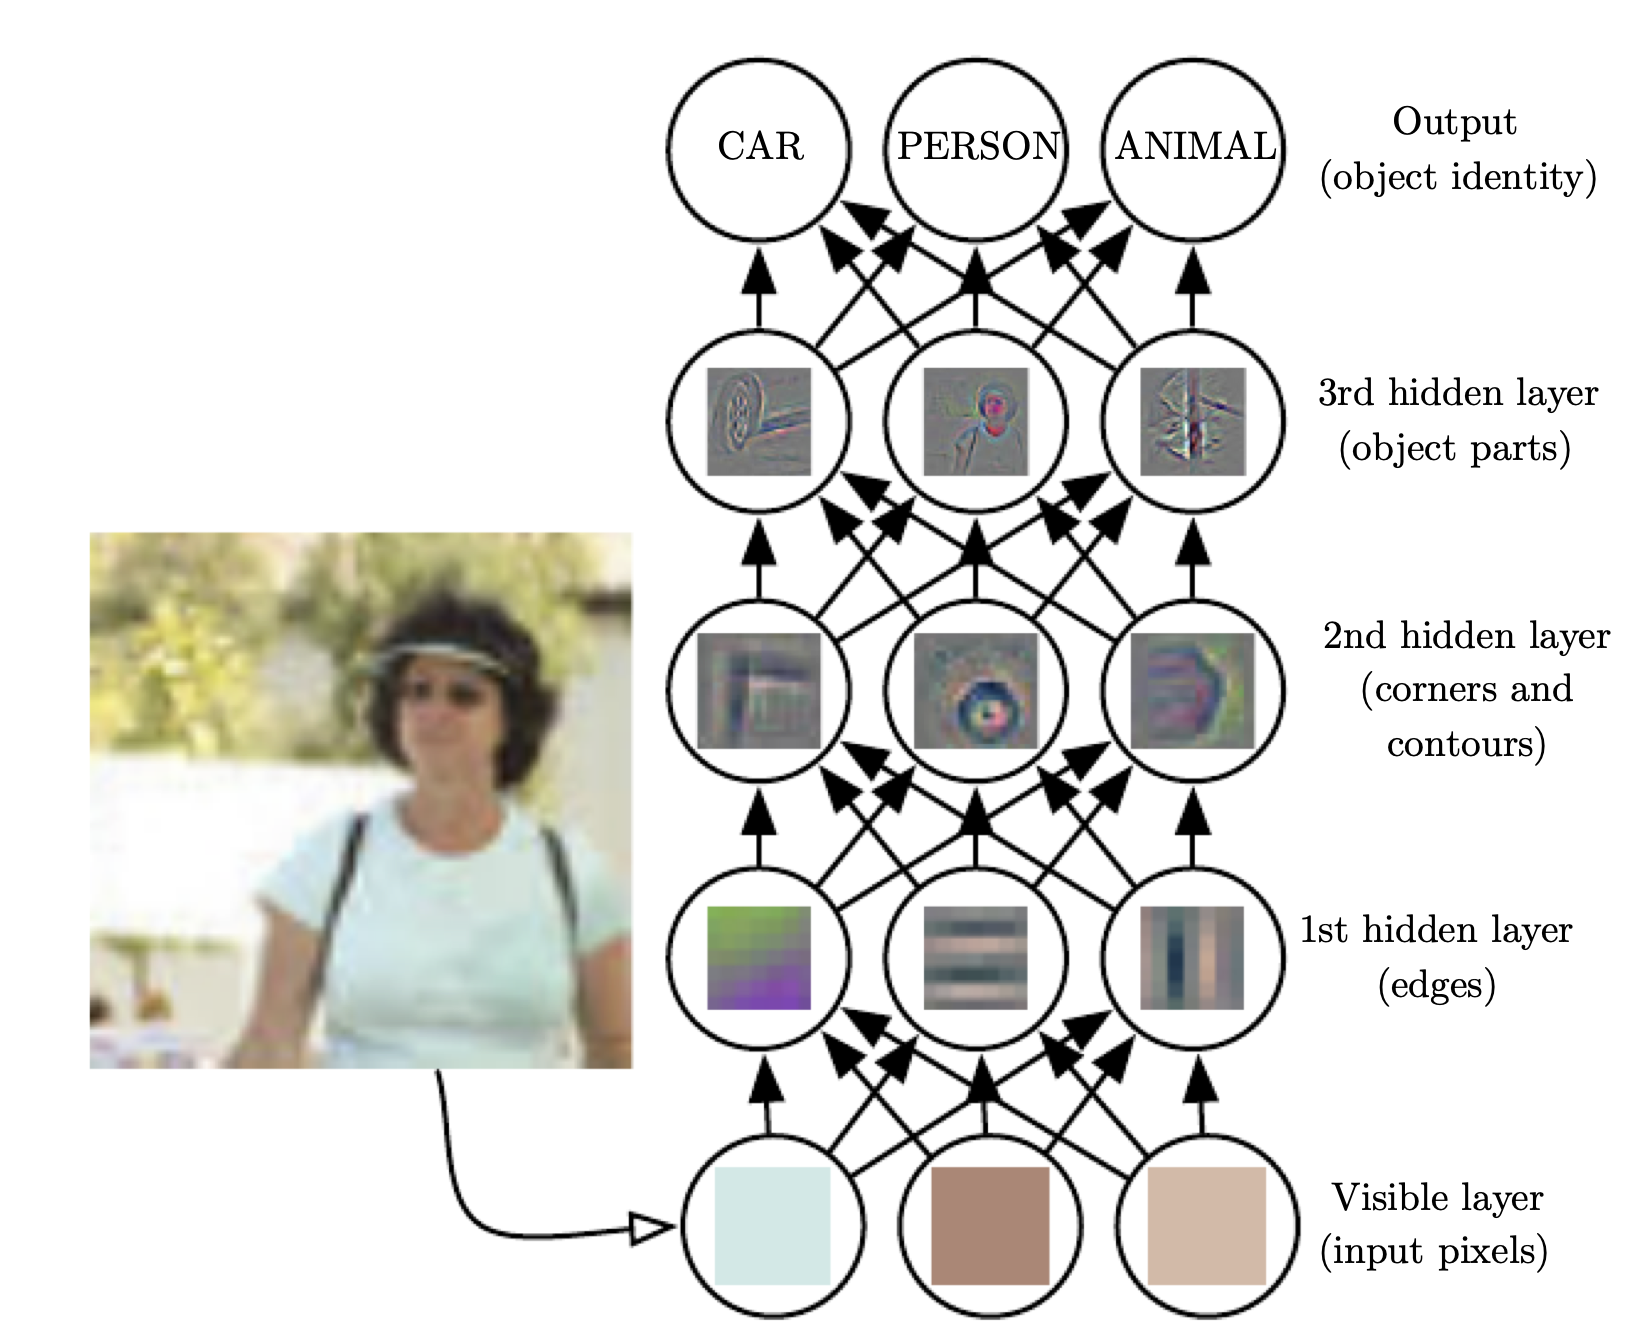
\includegraphics[width=0.8\textwidth]{fig/DL_fig_1_2_representations.png}
\caption{Learning representations for images (Goodfellow et al, 2017, Fig. 1.2)}
\end{figure}

}


\section{Convolution}
\frame{\sectionpage}


\frame{\frametitle{Convolution}

\begin{itemize}
\item Different definitions are common, one example:
\[
y(t) = \int x(\tau) k(t-\tau)d\tau = (x*k)(t)
\]
\item Inutuition: "Weighting together two functions"
\item In a convolutional layer:
\begin{enumerate}
\item $x(t)$: Input
\item $k(t)$: Kernel, filter, "feature"
\item $y(t)$: Output, feature map
\end{enumerate}
\end{itemize}
}


\frame{\frametitle{Discrete Convolution}

\begin{itemize}
\item If $t$ is discrete (as in a grid):
\[
y(t) = (x*k)(t) = \sum_{\tau=-\inf}^{\inf} x(\tau) k(t-\tau)
\]
\item In the case of images we have 2 discrete dimensions
\[
Y(i,j) = (X * K) \sum_{m} \sum_{n} X(m, n) K(i-m, j-n)
\]
\item Sometimes the cross-correlation is called convolution:
\[
Y(i,j) = (X * K) \sum_{m} \sum_{n} X(m, n) K(i+m, j+n)
\]
\begin{enumerate}
\item $X(i,j)$: Input (2D)
\item $K(i,j)$: Kernel, filter, "feature" (2D)
\item $Y(i,j)$: Output, feature map (2D)
\end{enumerate}
\end{itemize}
}



\frame{\frametitle{Convolution of Images: 2D}
\begin{figure}[h]
\centering
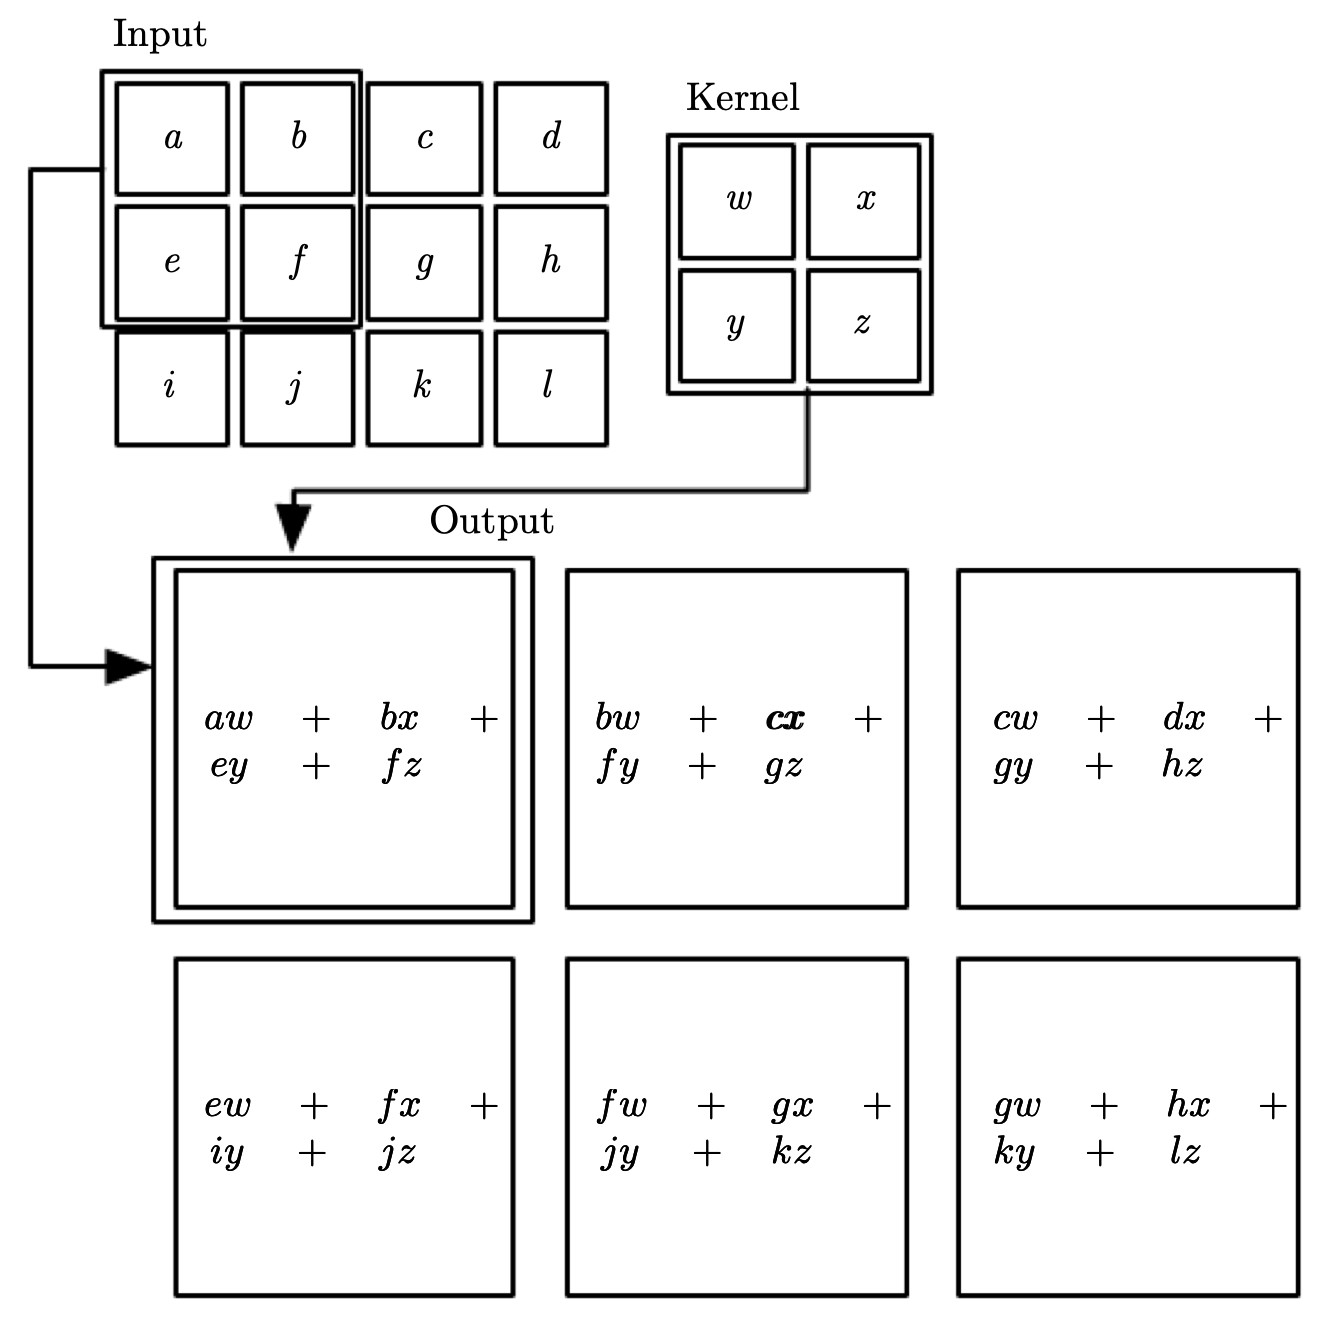
\includegraphics[width=0.8\textwidth]{fig/DL_fig_9_1_conv.png}
\caption{Convolution for an Image (Goodfellow et al, 2017, Fig. 9.1)}
\end{figure}
}

\frame{\frametitle{Convolution of images: Example}
\begin{figure}[h]
\centering
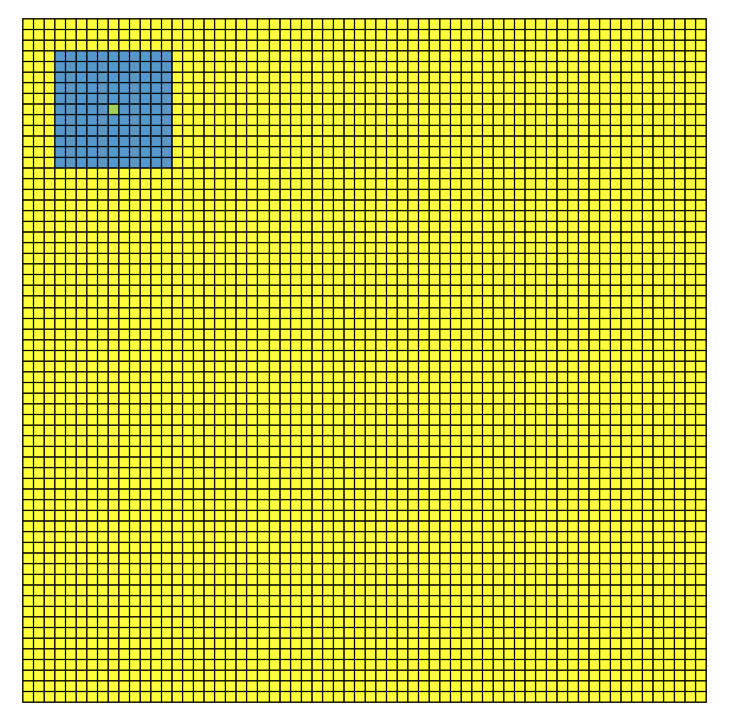
\includegraphics[width=0.8\textwidth]{fig/2d_conv_eklund.png}
\caption{Convolution example.}
\end{figure}
}

\frame{\frametitle{Convolution of images: Examples}
\begin{figure}[h]
\centering
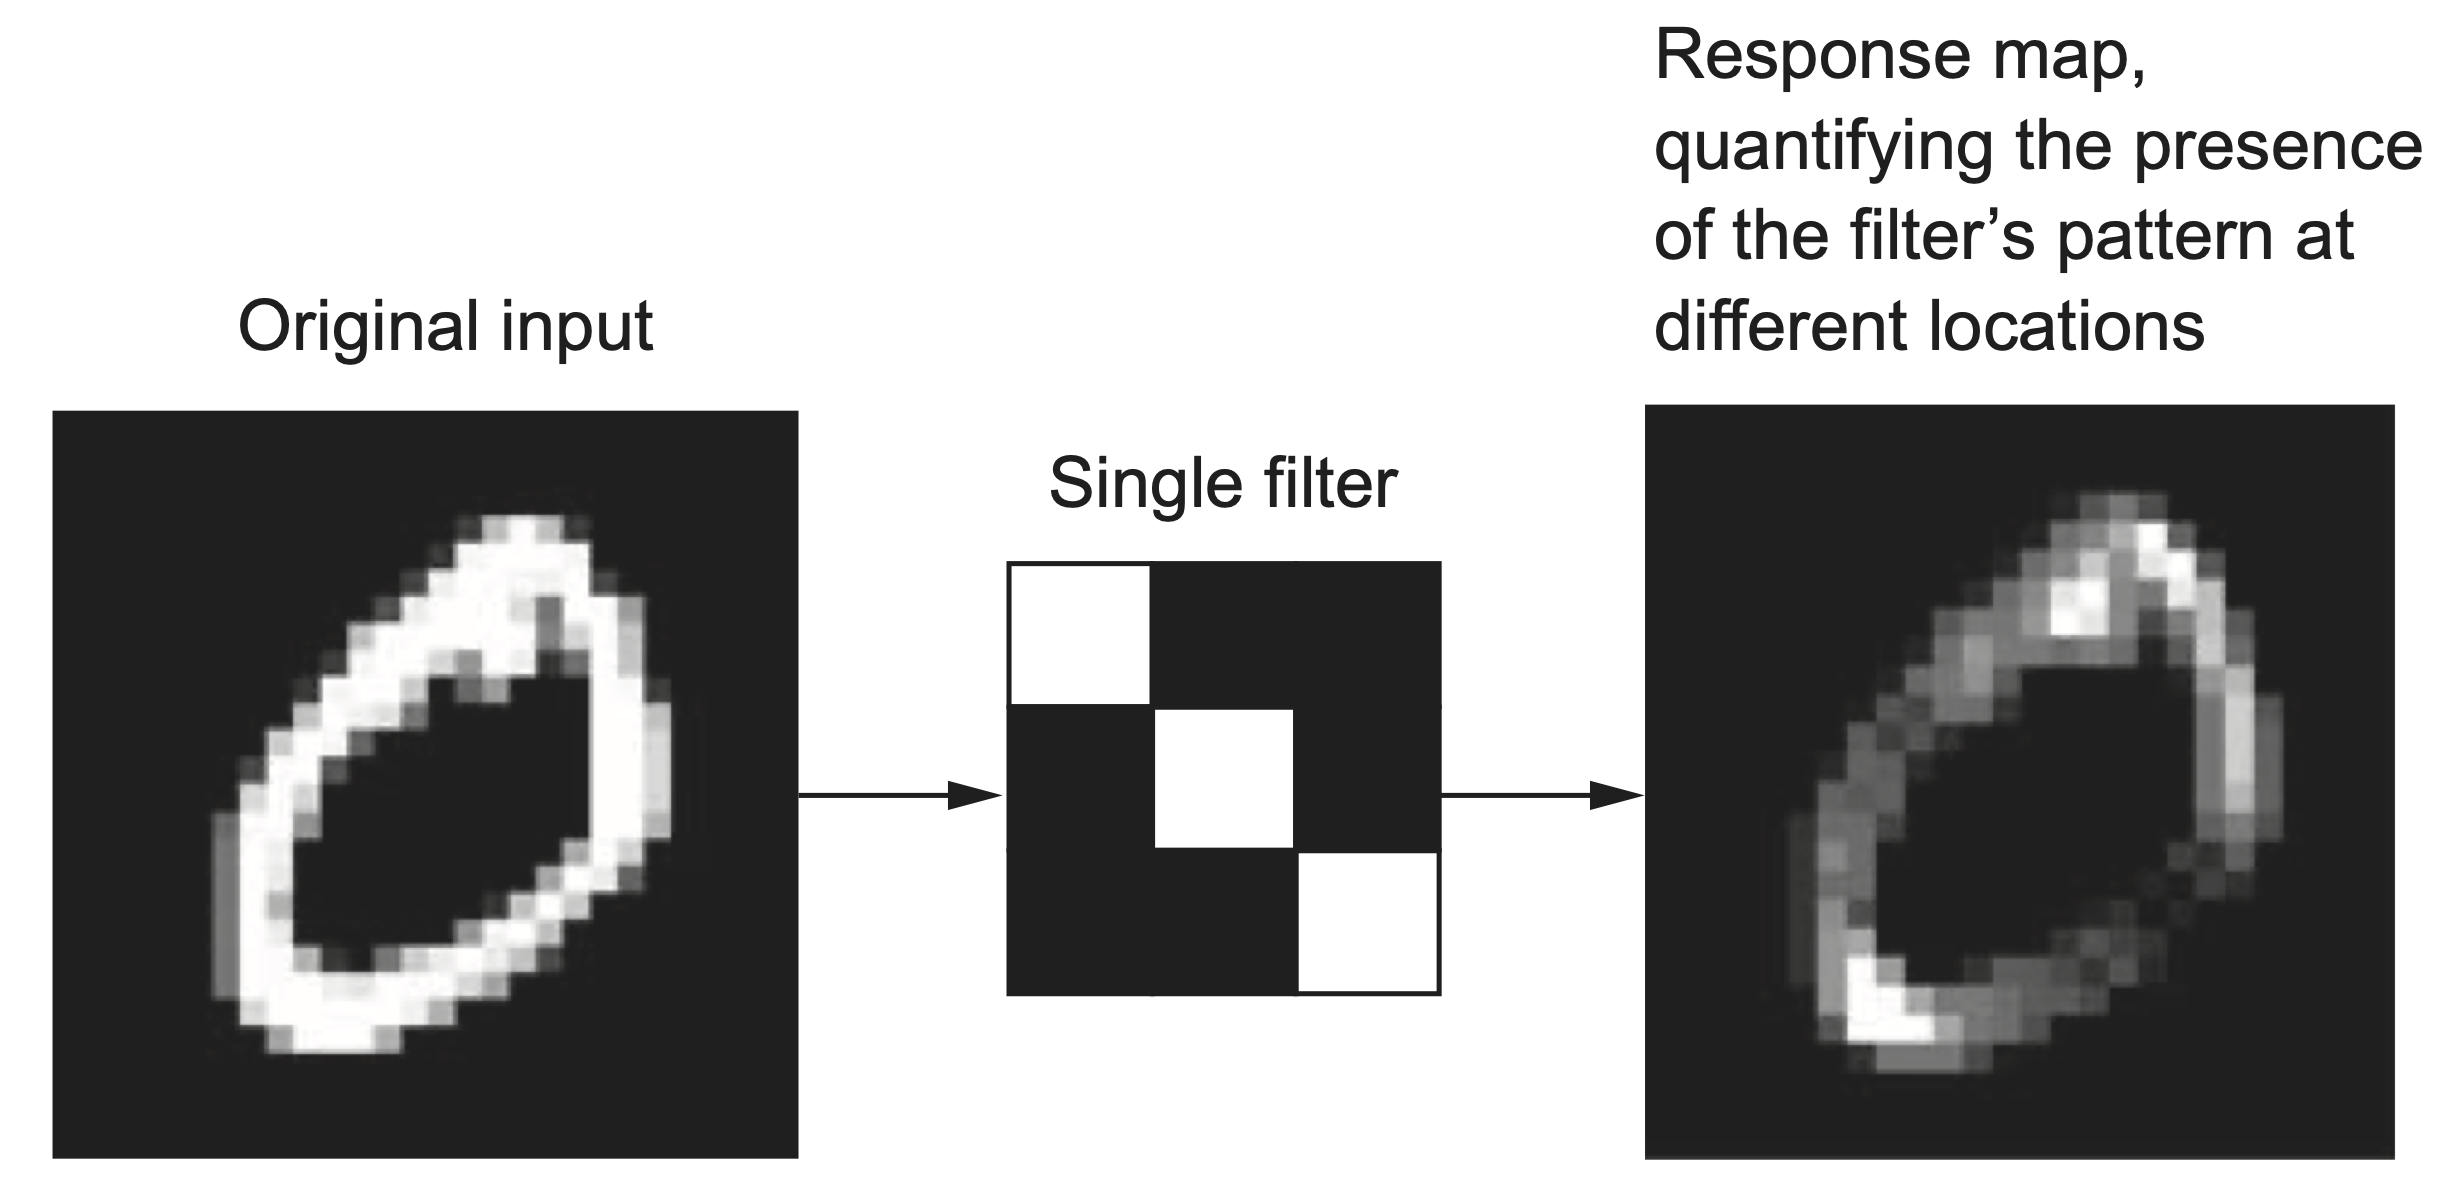
\includegraphics[width=0.8\textwidth]{fig/DLR_fig_5_3_conv_example.png}
\caption{Convolution for an Image (Chollet and Allaire, 2018, Fig. 5.3)}
\end{figure}

}


\frame{\frametitle{Convolution of images: Example}
\[
X=
  \begin{bmatrix}
    0 & 0 & 0 & 1 & 1 \\
    0 & 0 & 0 & 1 & 1 \\
    0 & 0 & 0 & 1 & 1 \\
    0 & 0 & 1 & 1 & 1
  \end{bmatrix}\,,
  K =
  \begin{bmatrix}
    -1 & 1 \\
    -1 & 1
  \end{bmatrix}
\]
\pause
\[
Y=
  \begin{bmatrix}
    0 & 0 & 2 & 0 \\
    0 & 0 & 2 & 0 \\
    0 & 1 & 2 & 0
  \end{bmatrix}\,,
\]
}




\section{Convolutional Neural Networks}
\frame{\sectionpage}

\frame{\frametitle{Convolutional Neural Networks}
\begin{figure}[h]
\centering
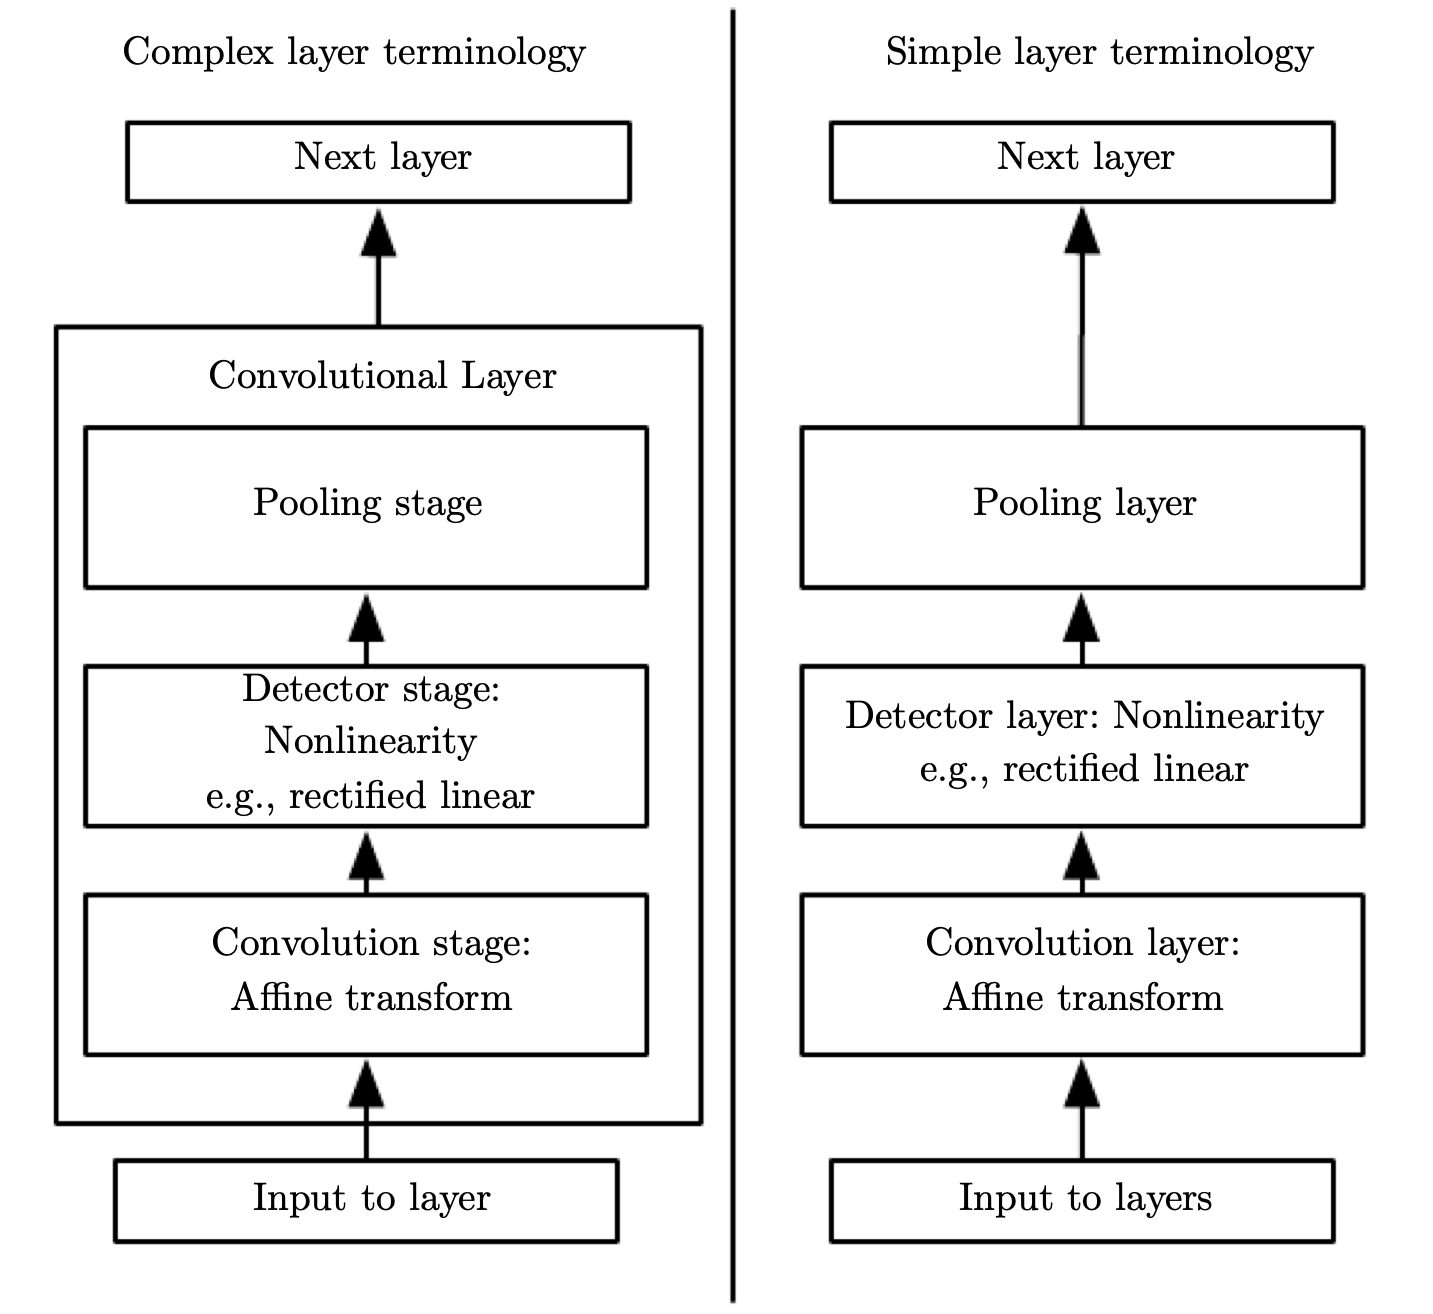
\includegraphics[width=0.8\textwidth]{fig/DL_fig_9_7_conv_layer.png}
\caption{Convolution layer (Goodfellow et al, 2018, Fig. 9.7)}
\end{figure}
}

\frame{\frametitle{Convolutional Neural Networks}

\begin{itemize}
\item Most convolutional neural networks have:
\begin{enumerate}
\item Many convolutional layers
\item More kernels higher up in the network
\item A classification head (usually a feed-forward neural network)
\end{enumerate}
\pause
\item Benefits:
\begin{enumerate}
\item Few(er) parameters (filters)
\item Captures {\color{uured} local structures}
\item Efficient computations\pause
\end{enumerate}
\item How to choose filters?
\begin{enumerate}
\item Before: {\color{uured} manually handcrafted}\pause
\item Now: {\color{uured} learn the filters}
\end{enumerate}

\end{itemize}

}

\subsection{The Convolution Layer}

\frame{\frametitle{Convolution layer}

\begin{itemize}
\item {\color{uured} Input}: Data or Feature Maps
\pause
\item {\color{uured} Parameters}:
\begin{itemize}
\item $N$ filters/kernels of size $m\times m$
\item $N$ bias terms (one per filter)
\end{itemize}
\pause
\item {\color{uured} Activation functions}: Applied element wise on feature maps
\pause
\item {\color{uured} Output}: Feature Maps
\pause
\item In Keras:\\
\texttt{layer\_conv\_2d(filters = 32, kernel\_size = c(3,3), activation = "relu", input\_shape = c(32,32,3))}
\end{itemize}

}

\frame{\frametitle{Padding}

\begin{itemize}
\item Handling {\color{uured} edges}
\item \emph{Padding}: add 0 around the image
\item Nessecary to {\color{uured} keep size} of feature maps
\end{itemize}

}


\frame{\frametitle{Padding}

\begin{figure}[h]
\centering
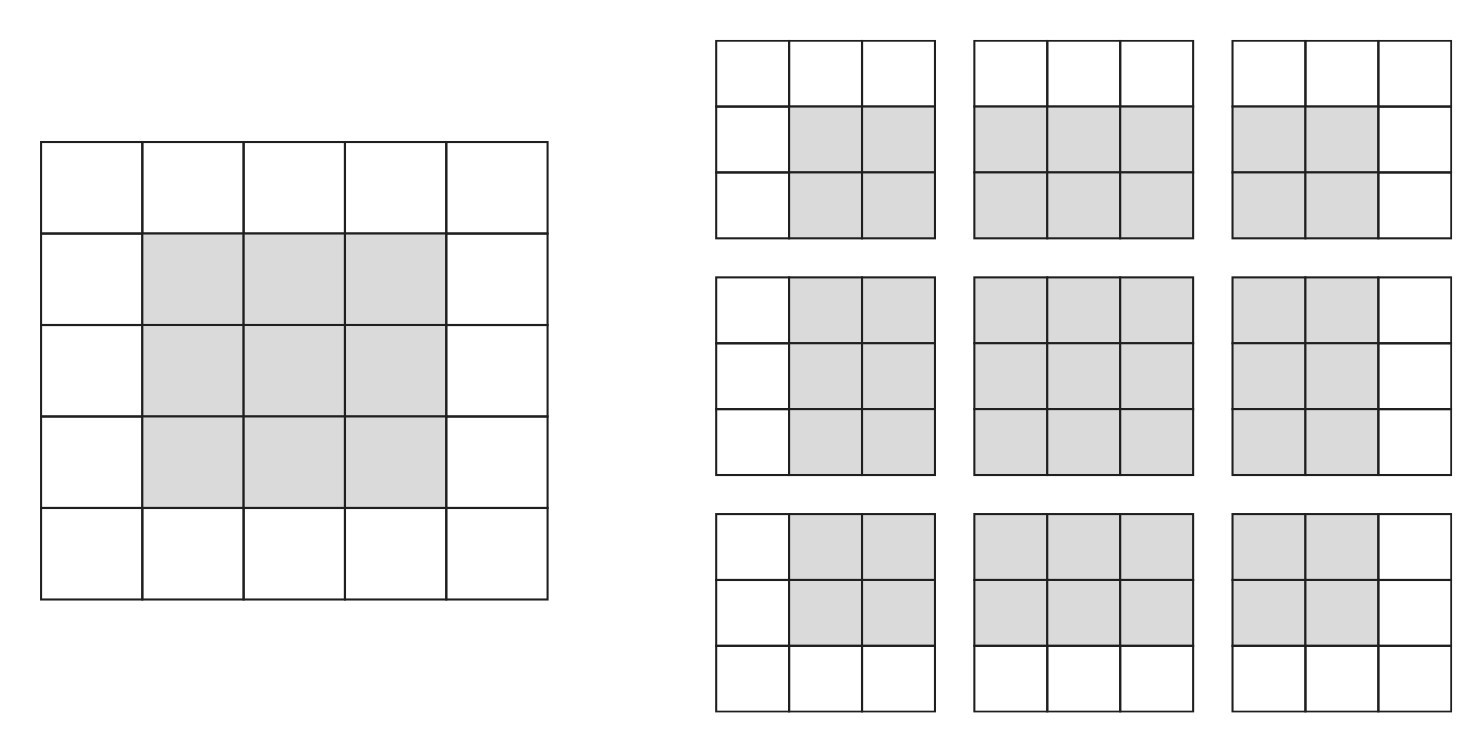
\includegraphics[width=0.8\textwidth]{fig/DLR_fig_5_5_valid.png}
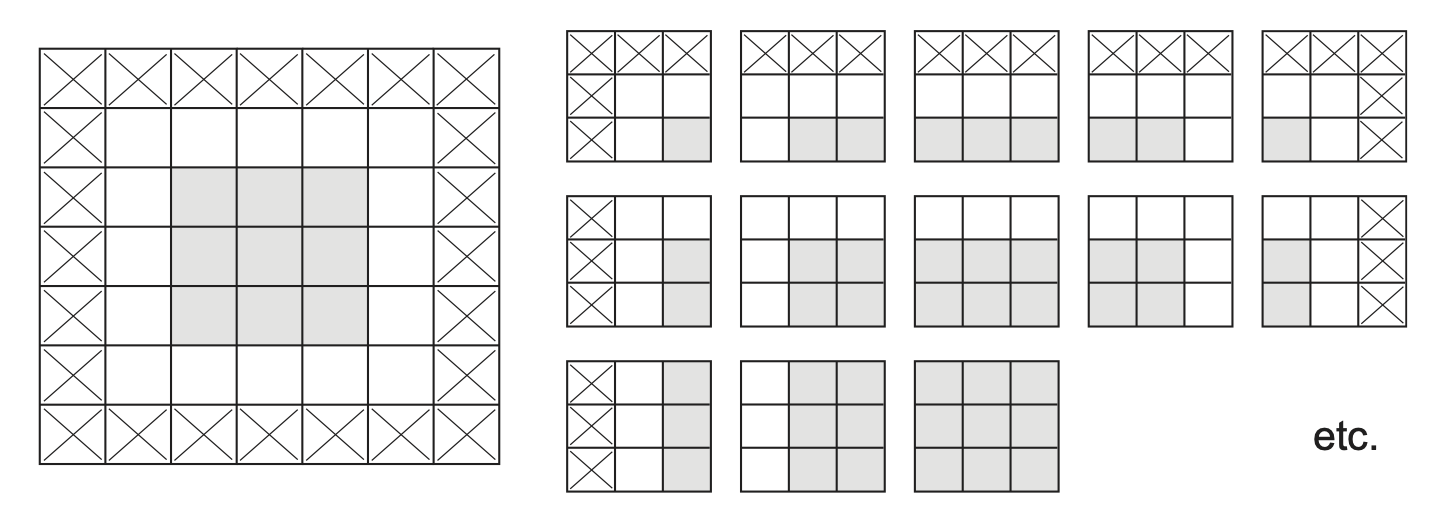
\includegraphics[width=0.8\textwidth]{fig/DLR_fig_5_6_padded.png}
\caption{Padding and valid edge handling (Chollet and Allair (2018), Fig. 5.5, 5.6)}
\end{figure}
}


\frame{\frametitle{Stride}

\begin{itemize}
\item {\color{uured} Skip} every $n$th pixel
\item Reduces the computations
\end{itemize}

\begin{figure}[h]
\centering
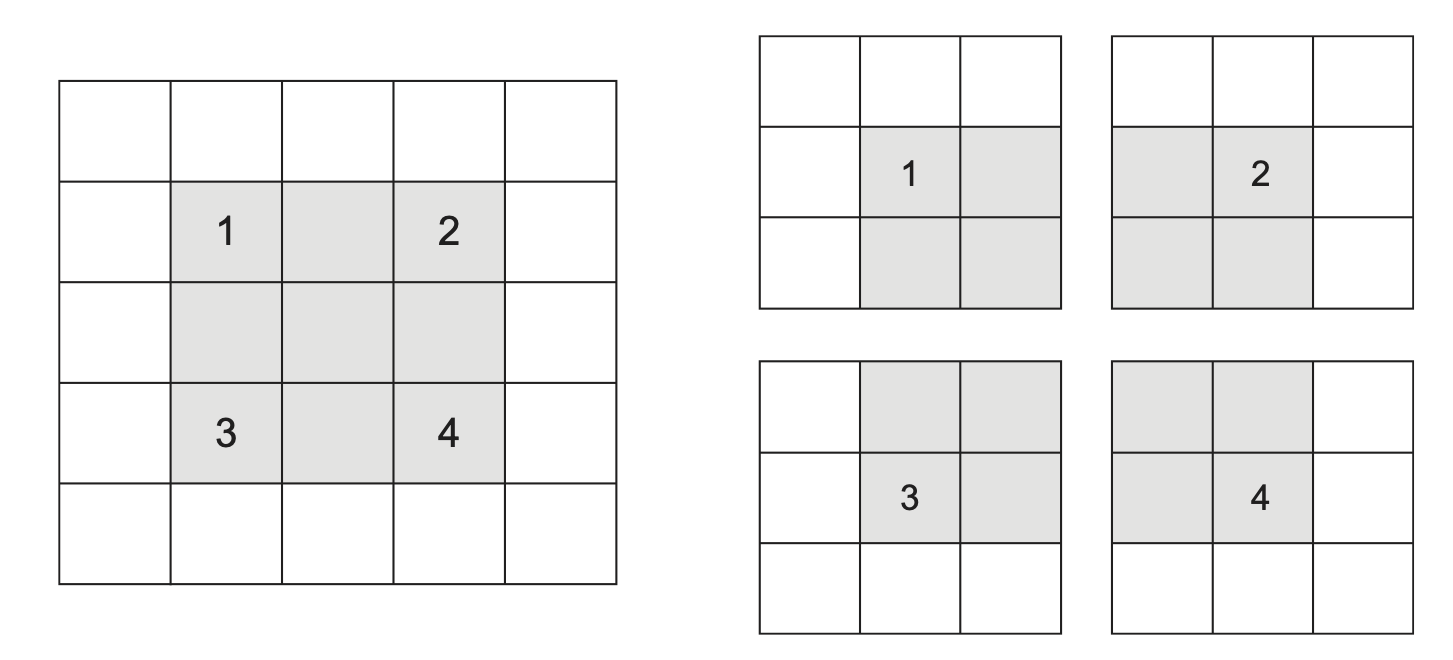
\includegraphics[width=0.8\textwidth]{fig/DLR_fig_5_7_2g2_stride.png}
\caption{Strides (Chollet and Allair (2018), Fig. 5.5, 5.6)}
\end{figure}
}


\frame{\frametitle{Why Convolution Layers?}

\begin{itemize}
\item Captures local spatial structure
\item Reduces the number of parameters (parameter sharing)
\begin{enumerate}
\item The number and size of filters
\item We use the same filters everywhere\pause
\end{enumerate}
\item Example: a 1 megapixel image ($1000 \times 1000$ pixels)
\begin{enumerate}
\item Dense network with 100 nodes: {\color{uured} 100M} parameters
\item CNN network with 100 $3\times 3$ filters: {\color{uured} 1000} parameters \\(900 from filters, 100 bias terms)
\end{enumerate}
\end{itemize}
}

\frame{\frametitle{Convolution Neural Nets}
\begin{figure}[h]
\centering
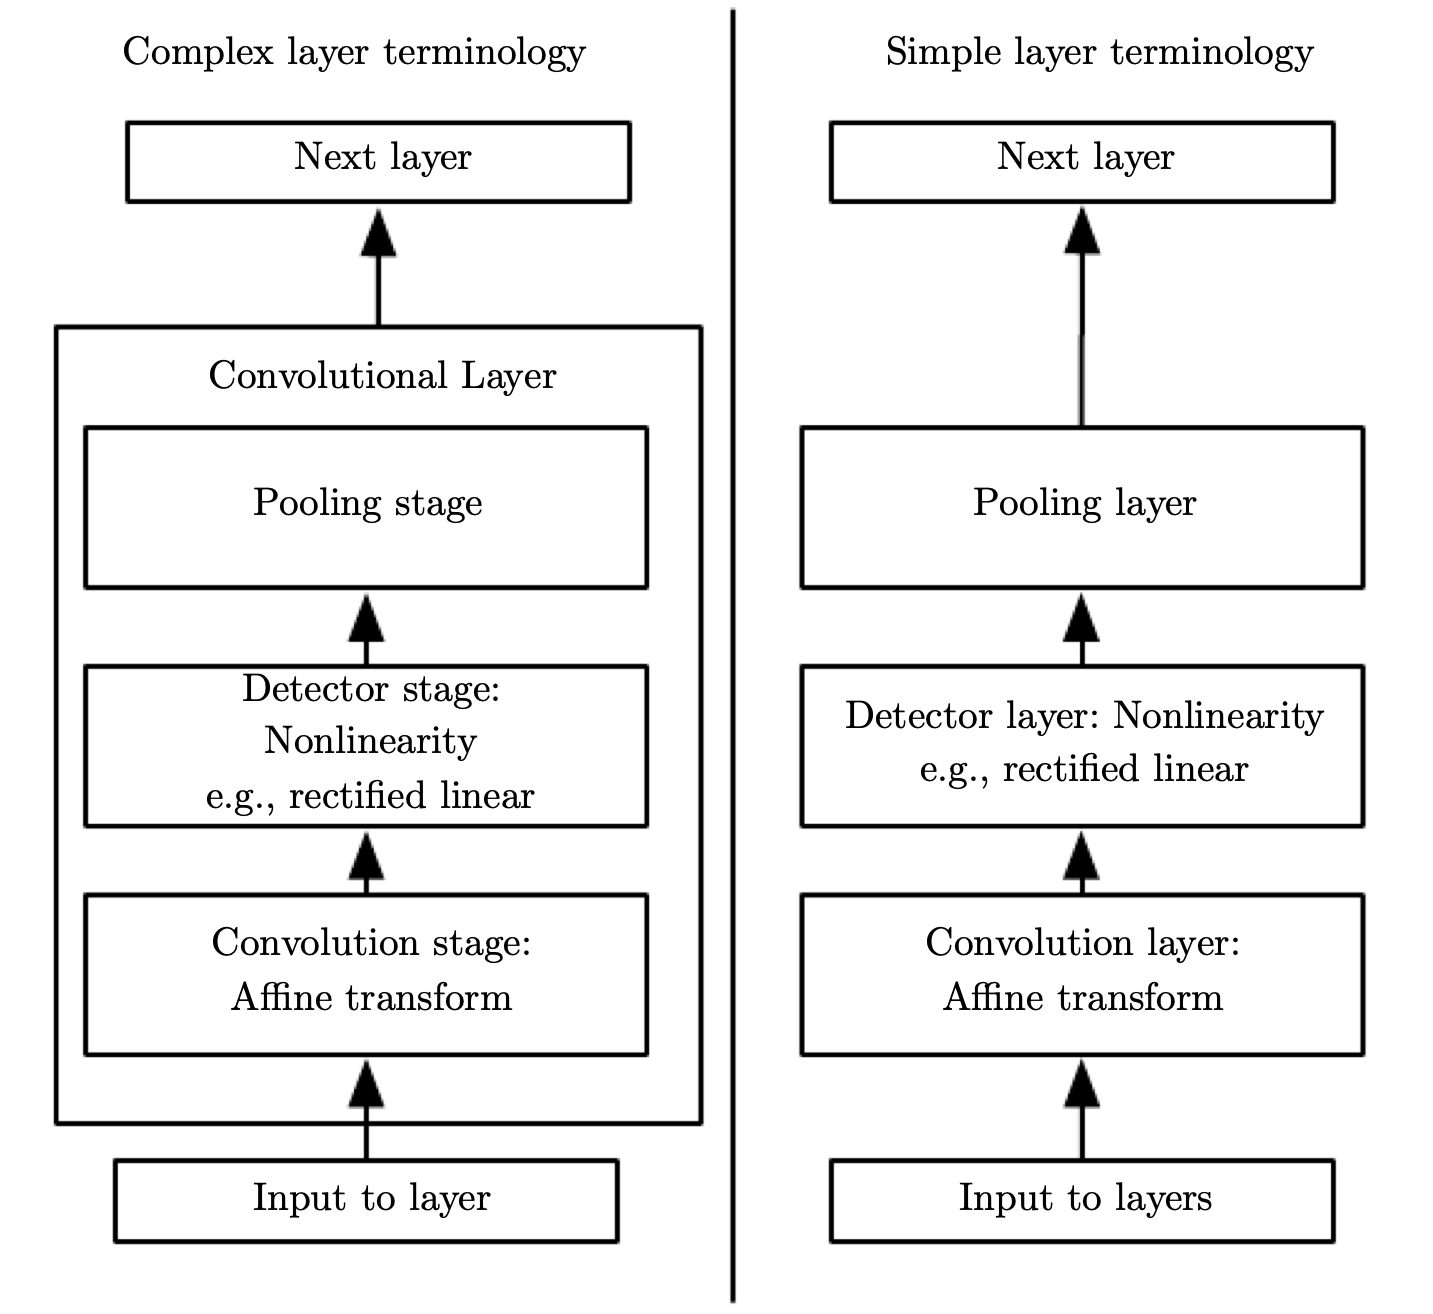
\includegraphics[width=0.8\textwidth]{fig/DL_fig_9_7_conv_layer.png}
\caption{Convolution layer (Goodfellow et al, 2018, Fig. 9.7)}
\end{figure}
}


\frame{\frametitle{Detector stage}

\begin{itemize}
\item Remember, in feed-forward networks: $\mathbf{h} = \sigma(\mathbf{X W}  + b)$
\item In CNN:
\begin{enumerate}
\item $\mathbf{W}$ is the filter\pause
\item $\mathbf{X}$ is the input feature map\pause
\item $\mathbf{X W}$ is the convolutional feature map\pause
\item $b$ is a bias (one per filter) \pause
\item $\sigma$ is the activation function (usually a ReLU)
\end{enumerate}
\end{itemize}

}

\subsection{The Pooling Layer}
\frame{\frametitle{Pooling layer}

\begin{itemize}
\item We take a function $f$ that return one value per pooling kernel\pause
\item Most commonly $f=\max$
\item Commonly a $2\times 2$ pooling kernel with stride 2
\item {\color{uured} Why?} Reduce the size of feature map, but keep the activation\pause
\item In Keras:\\
\texttt{layer\_max\_pooling\_2d(pool\_size = c(2, 2))}(
\end{itemize}

}

\frame{\frametitle{Max Pooling}

\begin{figure}[h]
\centering
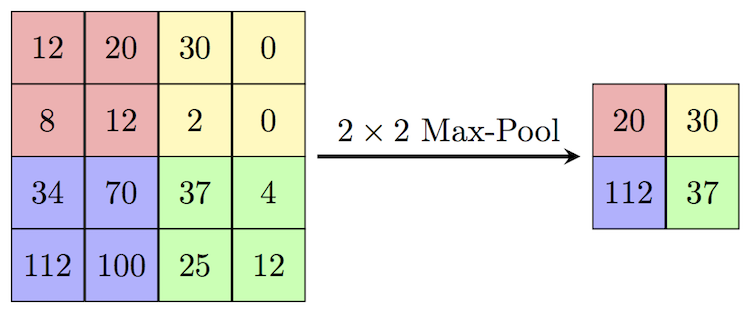
\includegraphics[width=0.8\textwidth]{fig/MaxpoolSample2.png}
\caption{Strides (Computer Science Wikipedia)}
\end{figure}
}

\frame{\frametitle{Using pooling to learn invariances}

\begin{itemize}
\item pooling over spatial positions: invariant to translation
\item pooling over different filters: invariant to transformations
\end{itemize}

\begin{figure}[h]
\centering
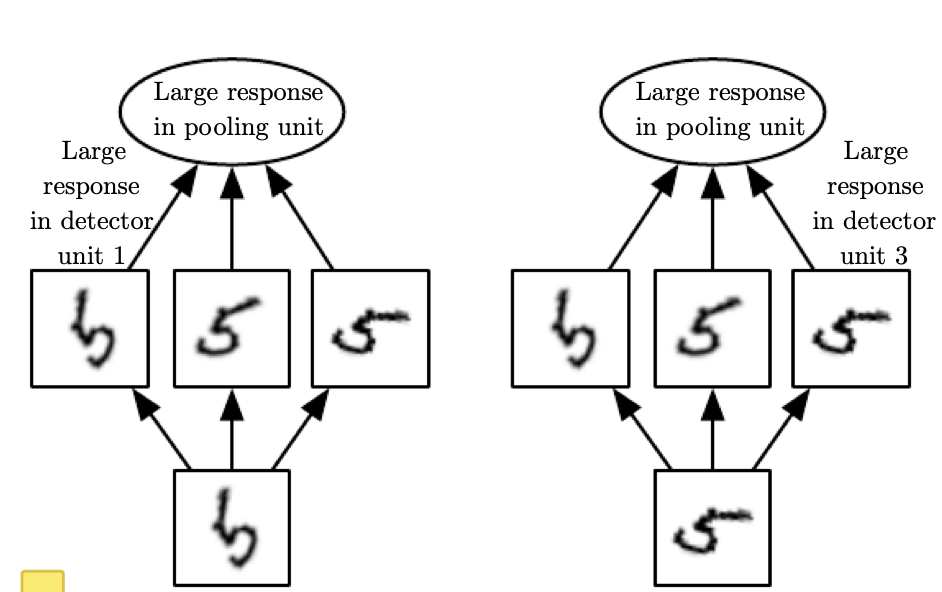
\includegraphics[width=0.7\textwidth]{fig/invariances.png}
\caption{Learning invariances (Goodfellow et al., 2017, Fig. 9.9)}
\end{figure}
}

\subsection{Regularization}

\frame{\frametitle{Data Augmentation}
\begin{figure}[h]
\centering
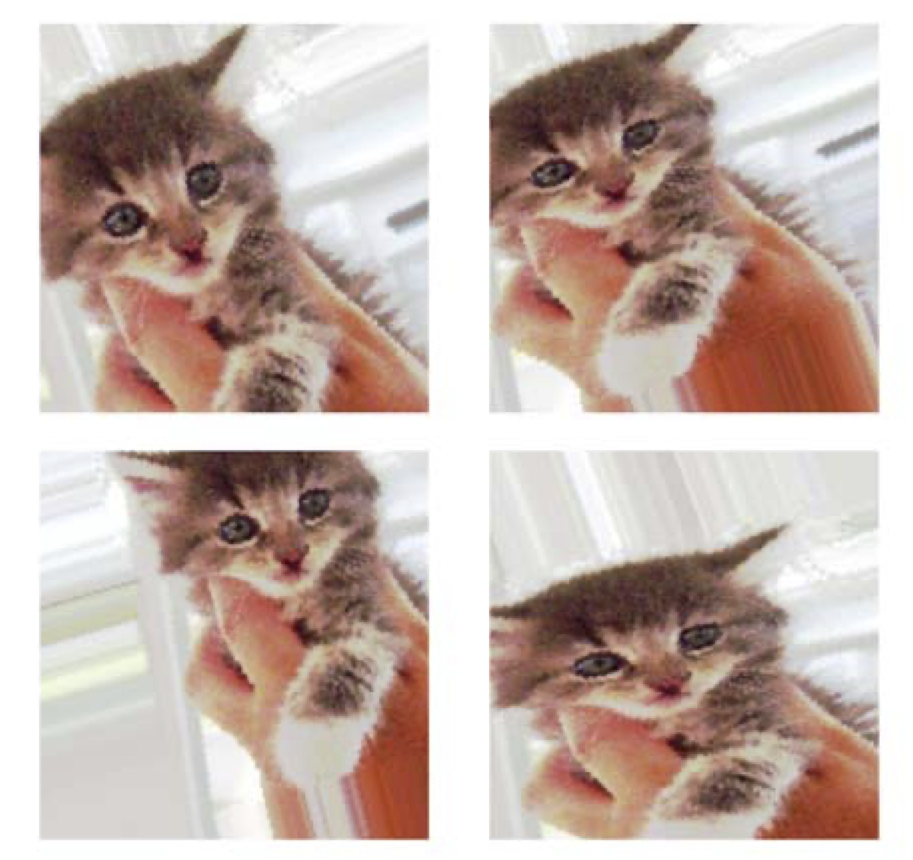
\includegraphics[width=0.6\textwidth]{fig/DLR_fig_5_10_data_augmentation.png}
\caption{Data Augmentation (Chollet and Allair, 2018, Fig 5.10)}
\end{figure}
\pause
\begin{itemize}
\item Can be done directly in Keras (data generator)
\end{itemize}
}


\subsection{Examples}

\frame{\frametitle{Popular CNN architectures}

\begin{itemize}
\item AlexNet (2012), 5 convolutional layers
\item VGG16 (2014), 16 convolutional layers
\item ResNet (2015), 152 convolutional layers
\end{itemize}
}

\frame{\frametitle{VGG16}

\begin{figure}[h]
\centering
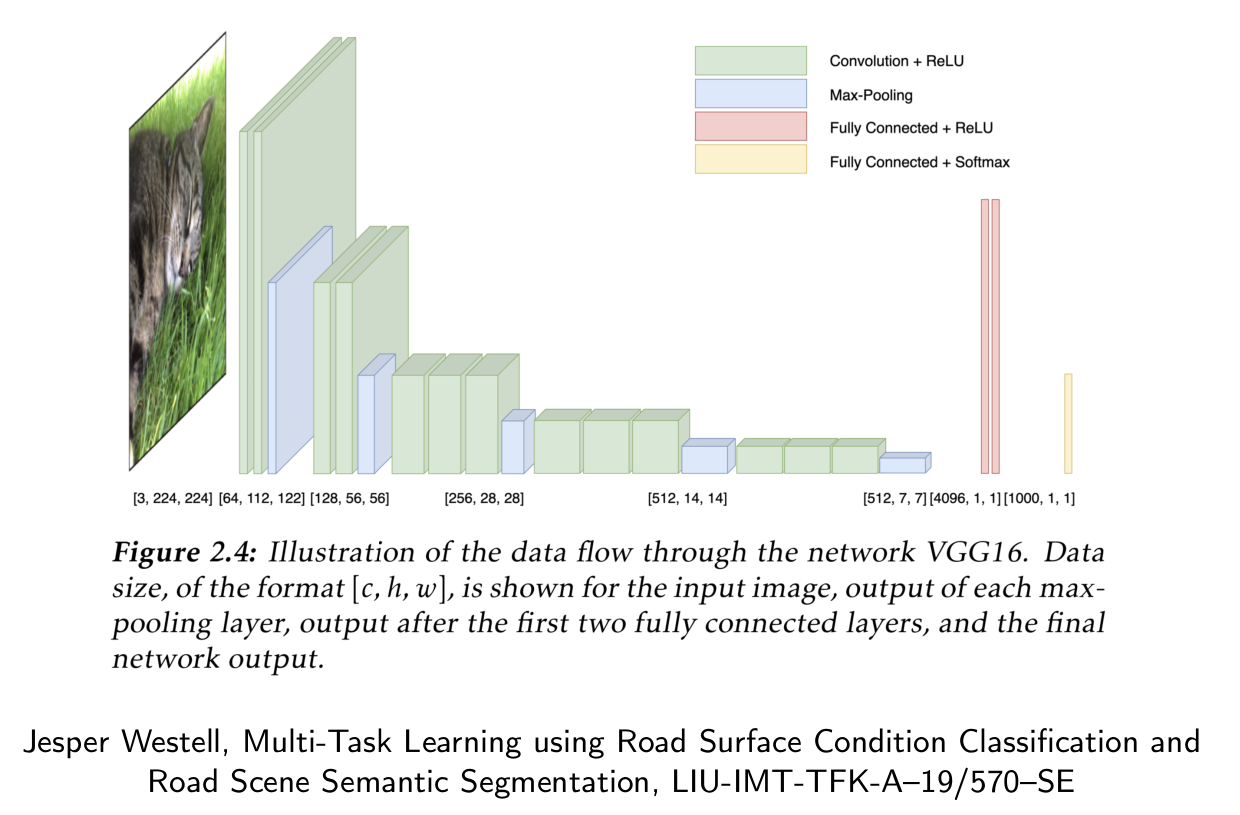
\includegraphics[width=0.9\textwidth]{fig/CNNVGG.png}
%\caption{Strides (Computer Science Wiki: "Max-pooling / Pooling")}
\end{figure}

}

\section{Transfer learning}
\frame{\sectionpage}

\frame{\frametitle{Transfer learning}

\begin{itemize}
\item "{\color{uured} Transfer knowledge} between problems"
\item In practice: Transfer/reuse {\color{uured} learned weights}\pause
\item A Bayesian perspective: A strong prior
\item Commonly: Use (large) pre-trained models for smaller problems
\item One of the main reasons for the success of (convolutional) neural networks\pause
\item Two types of transfer learning:
\begin{itemize}
\item Feature extraction
\item Fine Tuning
\end{itemize}
\end{itemize}

}



\frame{\frametitle{Learning Representations for Images}

\begin{figure}[h]
\centering
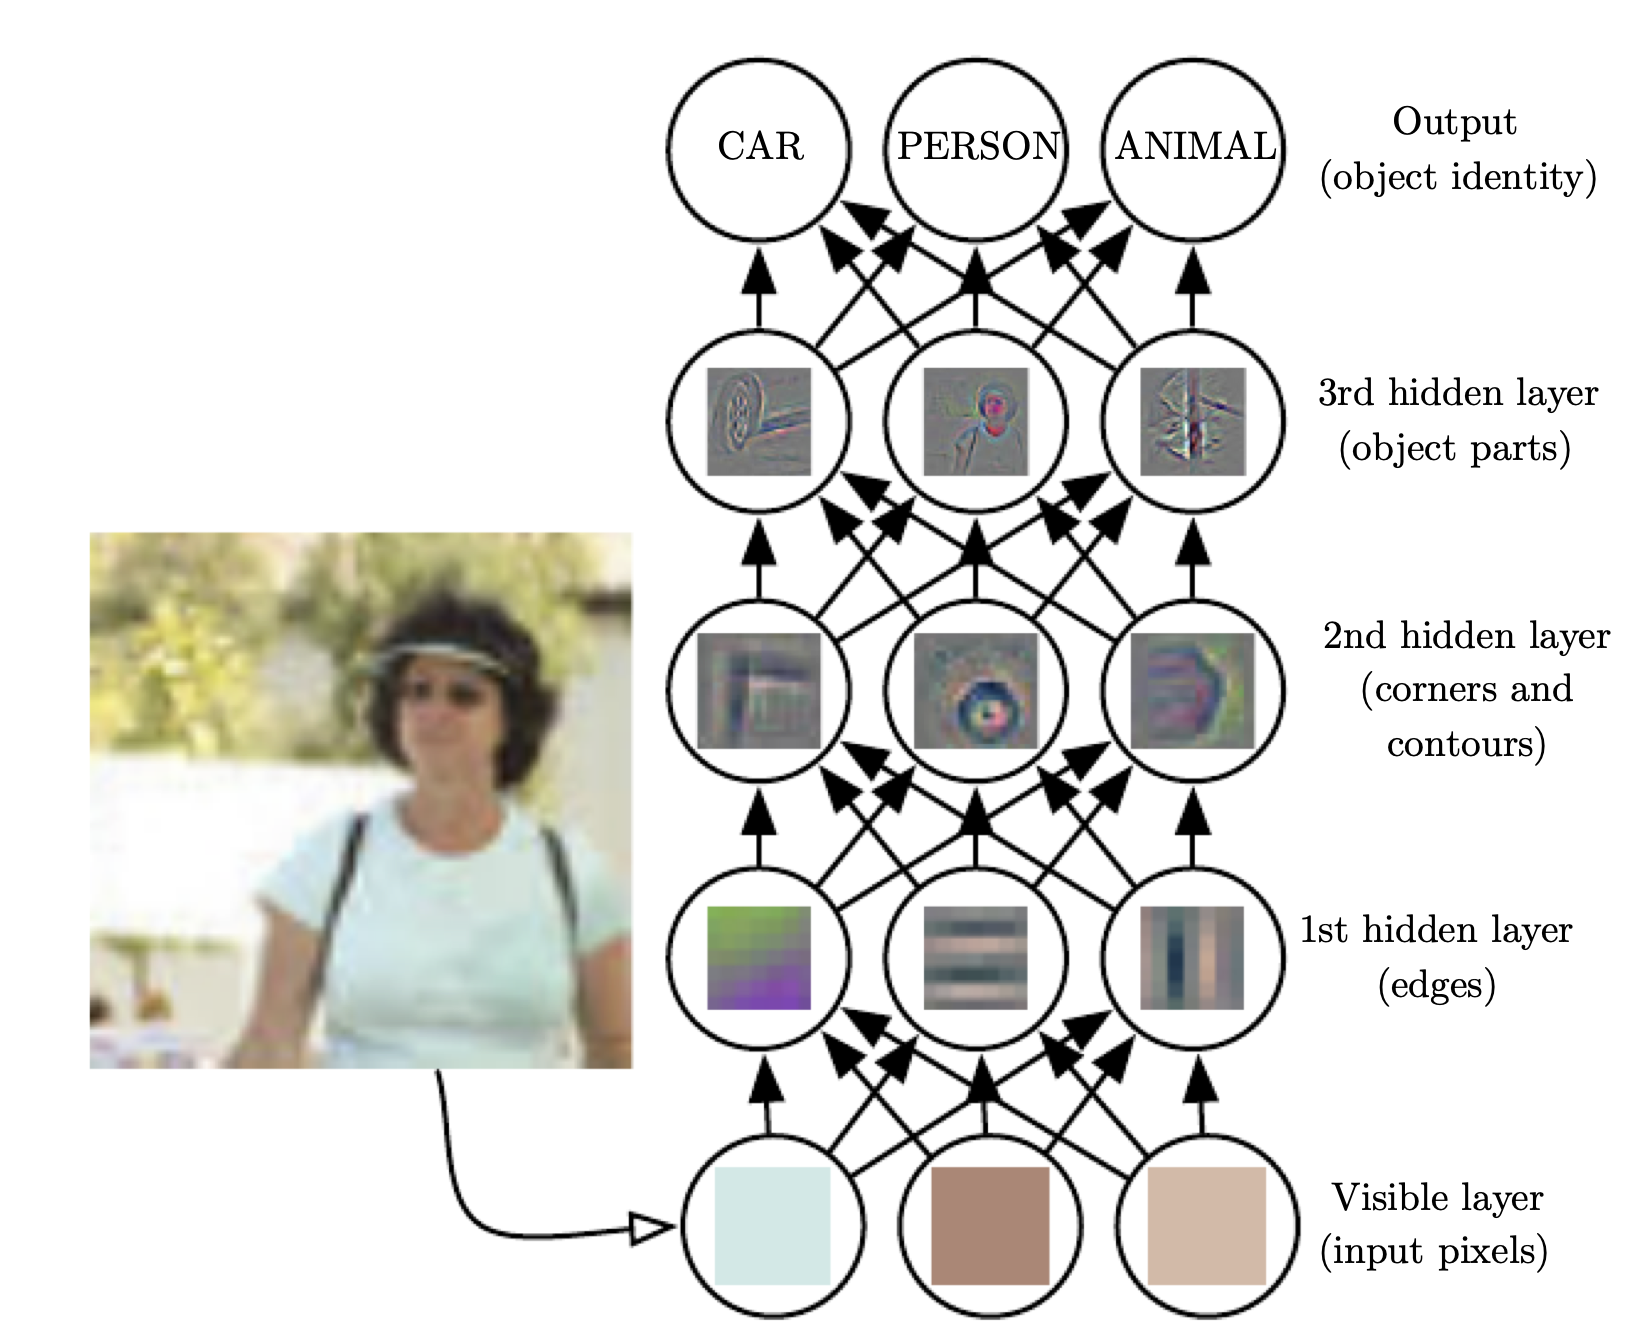
\includegraphics[width=0.8\textwidth]{fig/DL_fig_1_2_representations.png}
\caption{Learning representations can be crucial (Goodfellow et al, 2017, Fig. 1.2)}
\end{figure}

}


\frame{\frametitle{Feature Extraction}

\begin{figure}[h]
\centering
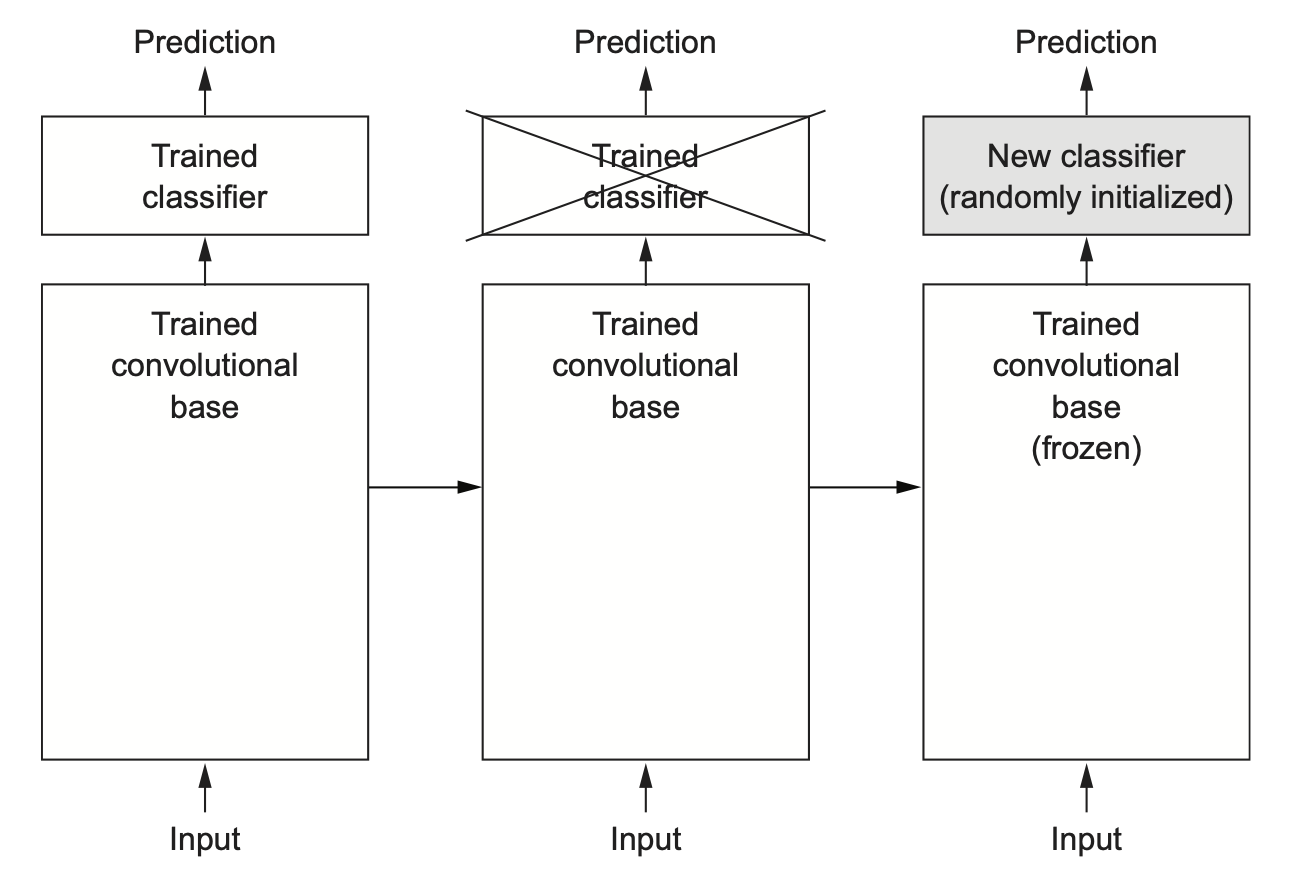
\includegraphics[width=0.8\textwidth]{fig/DLR_fig_5_12_feature_extract.png}
\caption{Using convnets as base for feature extraction (Chollet and Allair, 2018, Fig 5.12)}
\end{figure}

}

\frame{\frametitle{Fine-Tuning}

\begin{figure}[h]
\centering
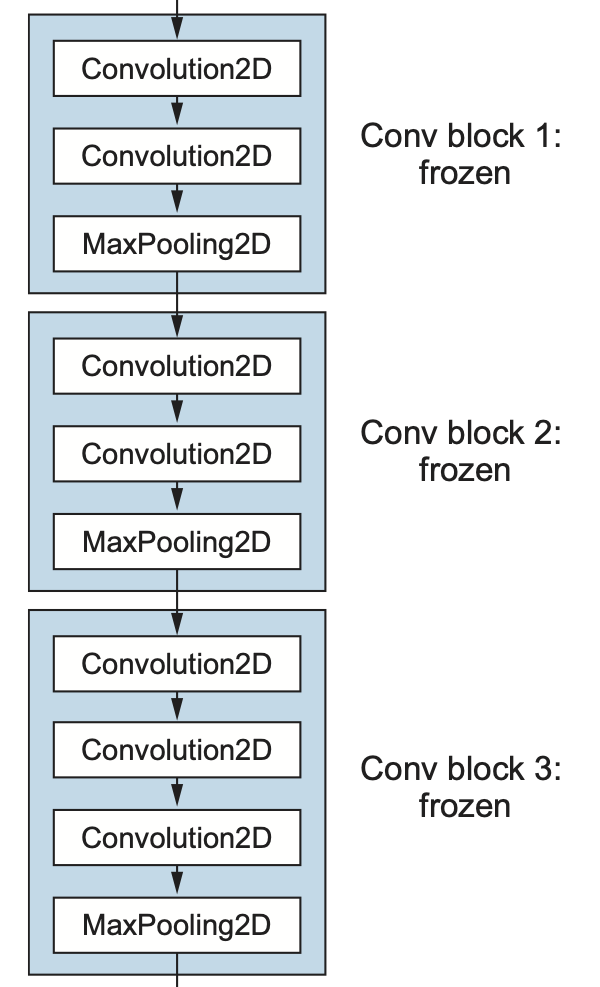
\includegraphics[width=0.45\textwidth]{fig/DLR_fig_5_15_a_fine_tune.png}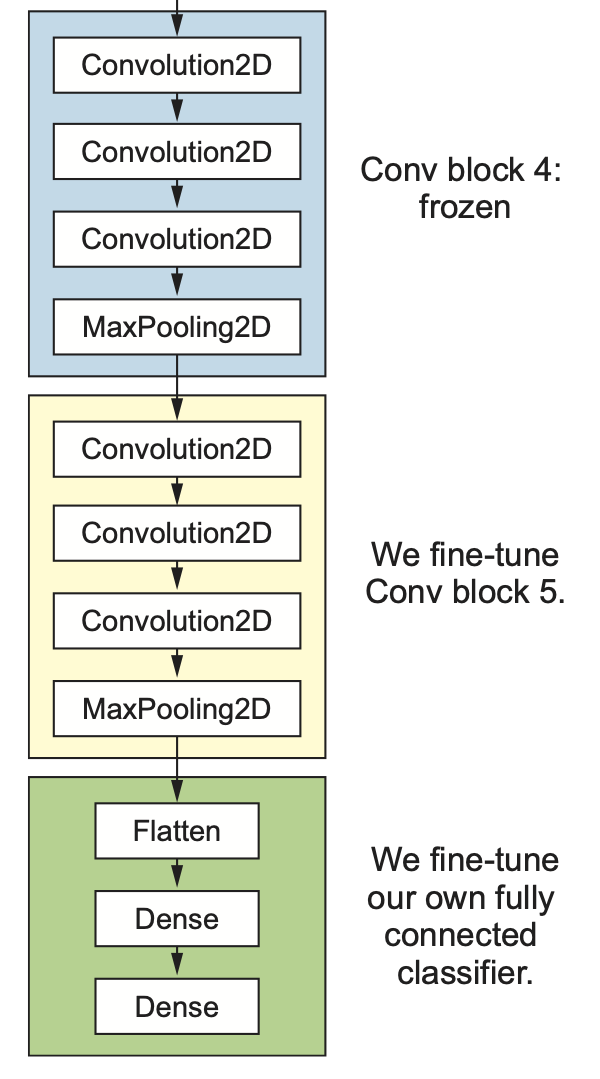
\includegraphics[width=0.45\textwidth]{fig/DLR_fig_5_15_b_fine_tune.png}
\caption{Finetuning a convolutional base (Chollet and Allair, 2018, Fig 5.15)}
\end{figure}

}

\section{Practical aspects}
\frame{\sectionpage}


\end{document}
